\section{Forms Module}\label{sec:01}

Forms allow users to perform a daily checkup of the equipment, assigned to them. A new Form Equipment can be added in the "Form Item" folder. A "Form" is currently under development, but it will contain a Collection of the "Form Items". A User can change the status (Accepted or not) of the Form Item on the Form Class web page. Every Form has the Status property. 

\subsection{Form Type Item}
In order 
Search results are displayed along with title, activity status and description of the relevant equipment classes, as displayed on \hyperref[sections/equipment/images/Fig.3]{Fig.~\ref*{sections/equipment/images/Fig.3}}.

    \begin{figure}[!htbp]
	\centering
	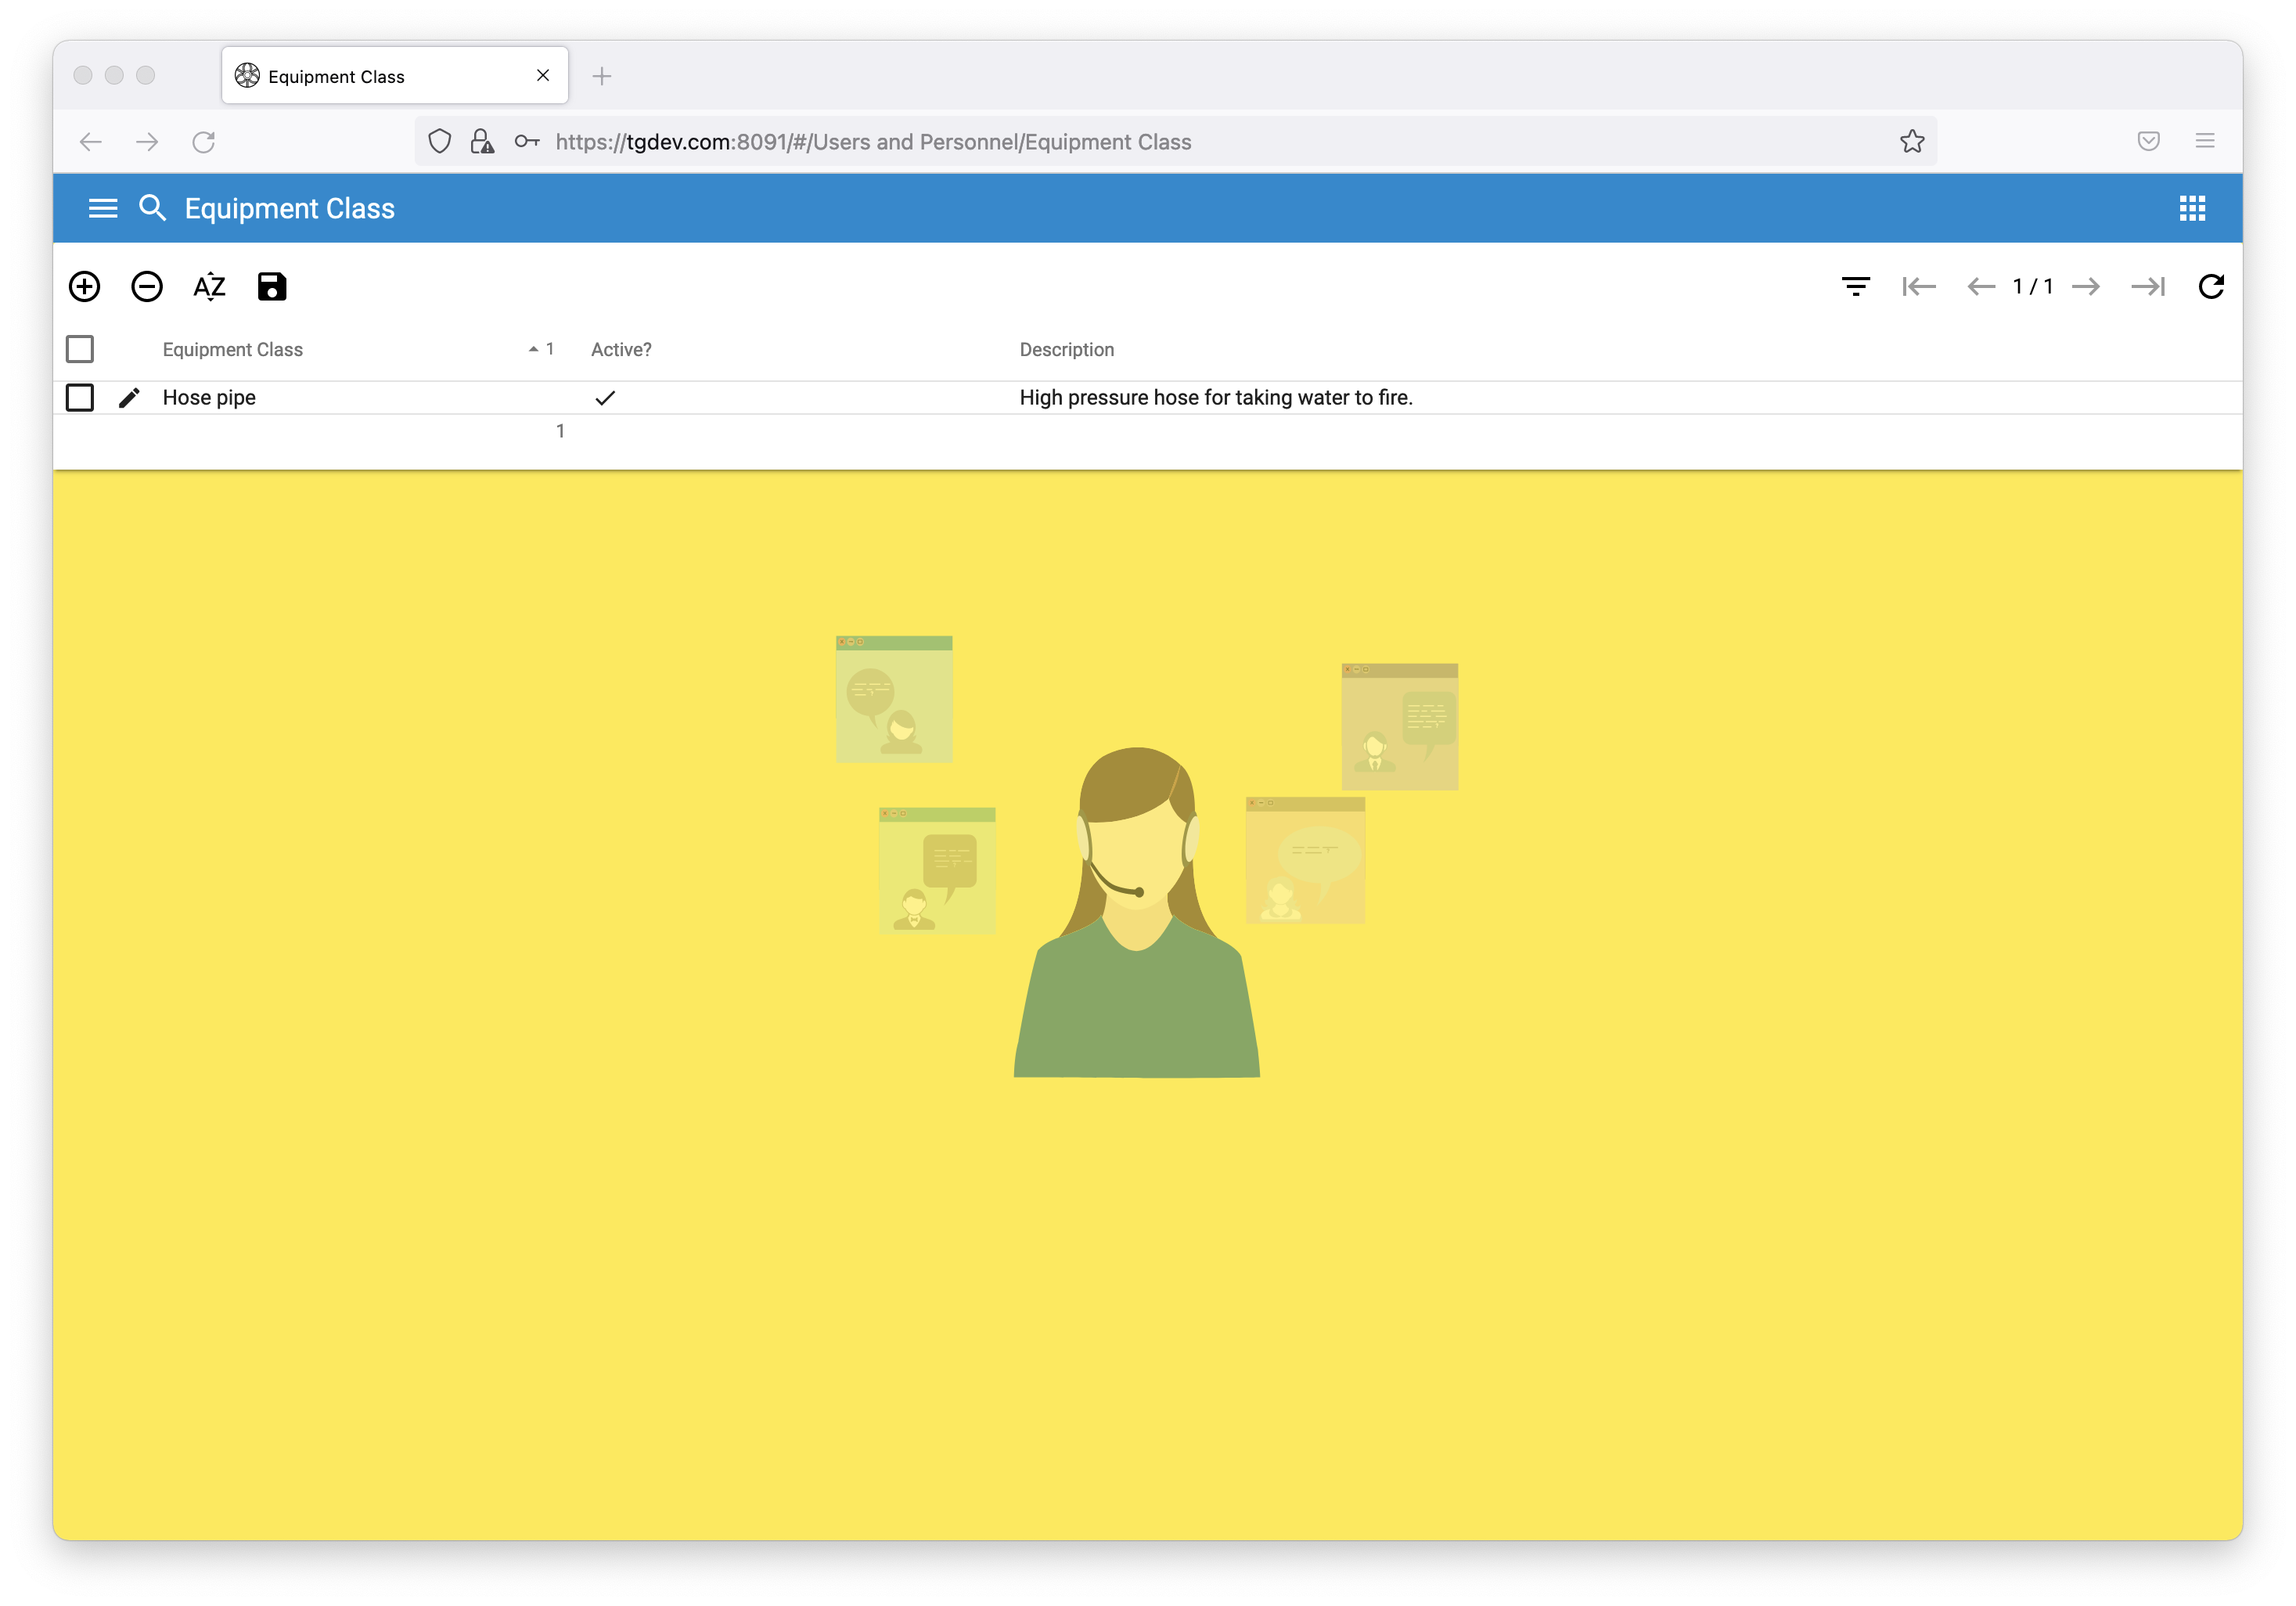
\includegraphics[width=0.95\linewidth]{sections/equipment/images/Fig.3.png}
	\caption{Equipment class search results.}\label{sections/equipment/images/Fig.3}
	\end{figure}
	
\newpage

\subsection{Form Item}
\subsection{For Type}
\subsection{Form Class}

